\setcounter{section}{3}
\section{Frequenzgang und Polstellenlage}
\begin{tcolorbox}[colback=white!10!white,colframe=green!30!black,title=PT$_2$ - Glied] 
    \begin{figure}[H]
        \begin{minipage}{.3\textwidth}
            \centering
            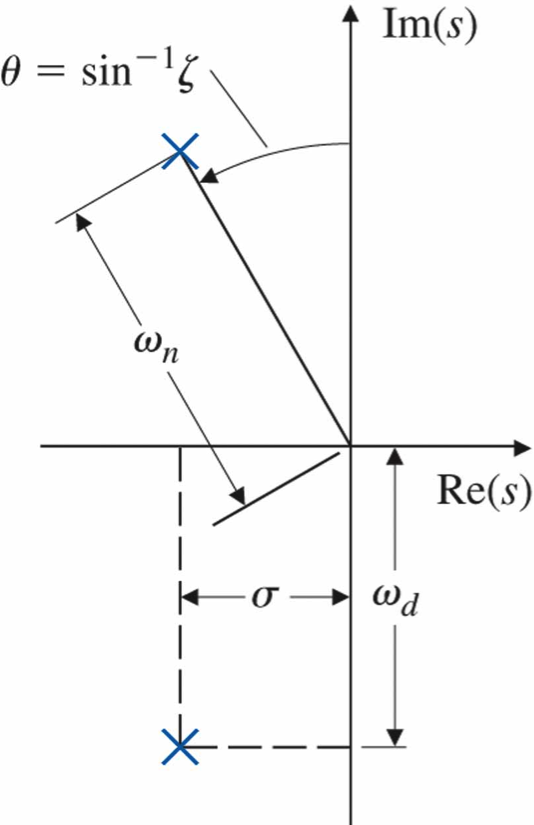
\includegraphics[width=1\textwidth]{images/winkel}
        \end{minipage}%
        \hspace{1cm}
        \begin{minipage}{.6\textwidth}
            Instabilität beginnt in der rechten Halbebene. 
            
            Für die  \textbf{Dämpfung} gilt, je kleiner der Winkel $\theta$, desto kleiner ist die Dämpfung: \begin{align*}
                \theta = \arcsin{\zeta}
            \end{align*}
        \end{minipage}%
        
    \end{figure}
    \textbf{Charakteristische Gleichung:} $s^2+2*\zeta*\omega_n*s+\omega_n^2$
\end{tcolorbox}

\begin{tcolorbox}[colback=white!10!white,colframe=green!30!black,title=Auswirkung der NST und Polenlage] 
    \begin{figure}[H]    
            \centering
            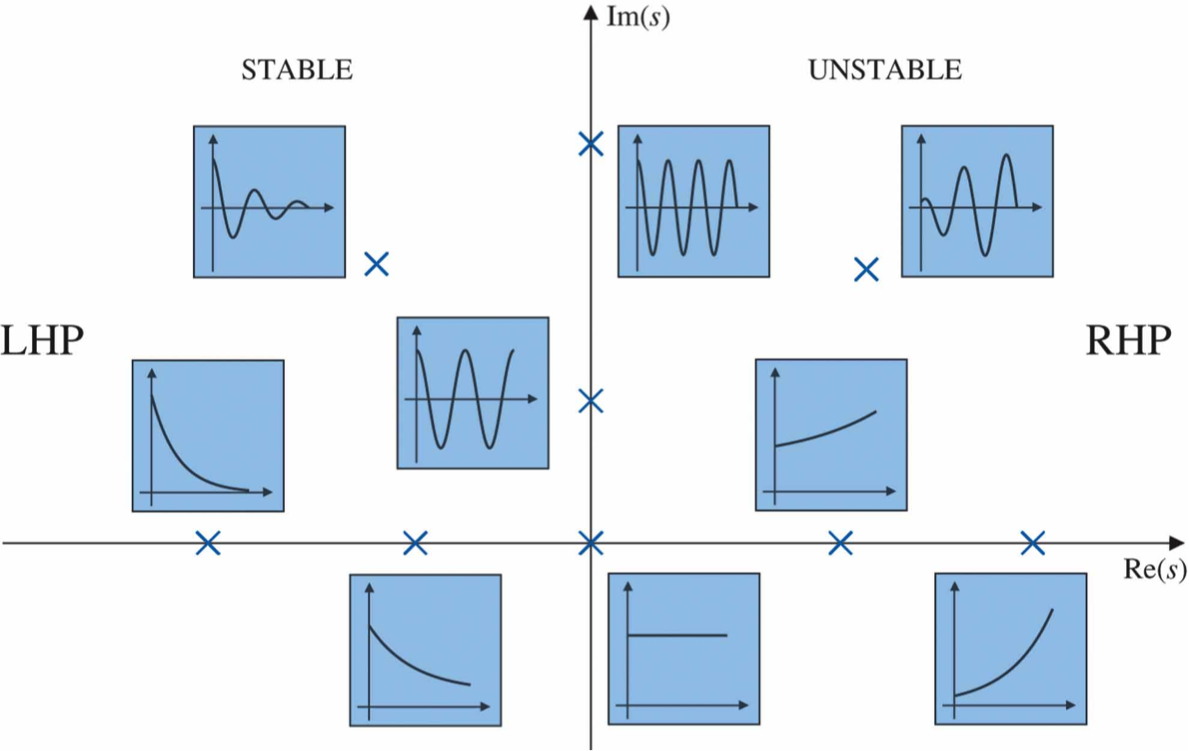
\includegraphics[width=1\textwidth]{images/lageAntwort}
    \end{figure}
\tcblower
    \textbf{Polstelle (reell + komplexes Polpaar)}
    \begin{table}[H]
        \centering
        \begin{tabular}{ccc}
            \hline Re & Im & Auswirkung \\ 
            \hline $<$ 0 & = 0 & stabil - keine Schwingung \\ 
            \hline $>$ 0  & =0 & instabil - keine Schwingung \\ 
            \hline $=0$ & =0 & instabil - keine Schwingung \\ 
            \hline\hline $< 0$ & $\not =$ & stabil - Schwingung \\ 
            \hline $> 0$  &  $\not =$ & instabil - Schwingung \\ 
            \hline = 0  & $\not =$ & Dauerschwingung \\ 
            \hline 
        \end{tabular} 
    \end{table}
    \textbf{Nullstelle:}
    \begin{table}[H]
        \centering
        \begin{tabular}{p{2cm}p{3cm}}
            \hline $< = 0 $ & minimalphasiges System (evtl. Überschwung) \\ 
            \hline $> = 0 $ & nichtminimalphasiges System (Systemantwort erst entgegen der Sprunganregung) \\ 
            \hline $= 0 $ & $lim_{t\rightarrow\infty}y(t)\rightarrow 0$ \\ 
            \hline 
        \end{tabular} 
    \end{table}
\end{tcolorbox}
\begin{tcolorbox}[colback=white!10!white,colframe=green!30!black,title=Kenngrößen] 
    \begin{figure}[H]
        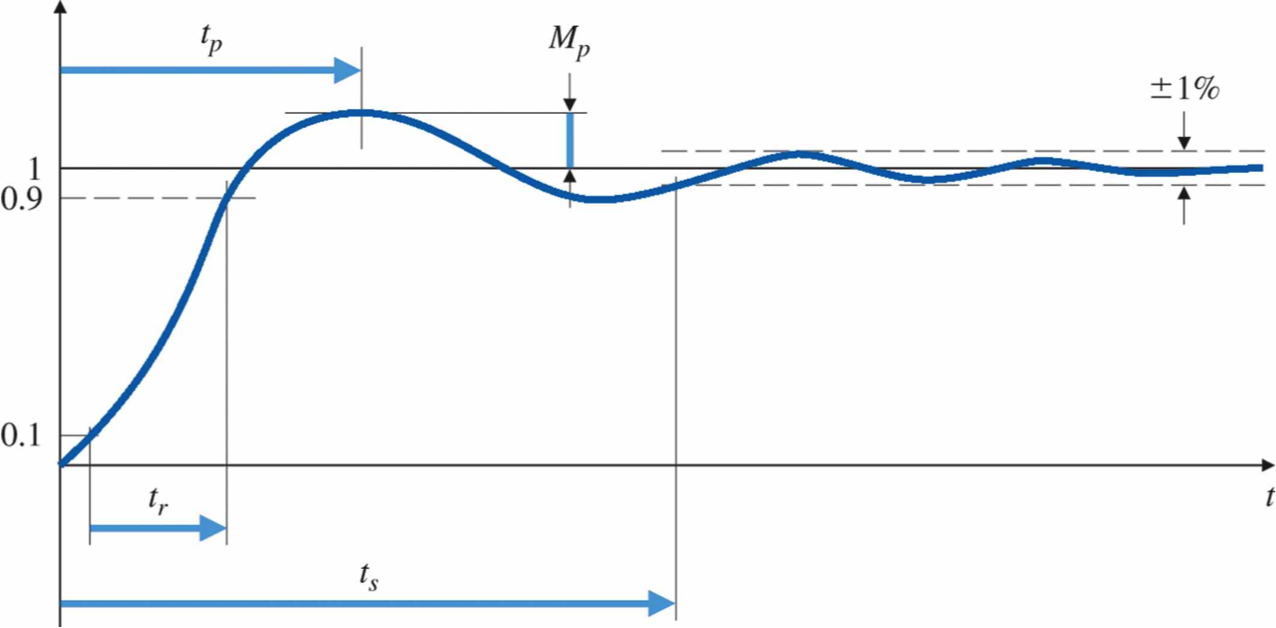
\includegraphics[width=1\linewidth]{images/numb}
    \end{figure}
\begin{minipage}{.45\textwidth}
        Steigzeit (0,1 - 0,9):
    \begin{align*}
        t_r &\approx \frac{1,8}{\omega_n} 
    \end{align*}
\end{minipage}
\begin{minipage}{.45\textwidth}
 Einschwingzeit (Abklang auf) $\pm 1\%$
 \begin{align*}
 t_s  &= \frac{4,6}{\zeta\omega_n} = \frac{4,6}{\sigma}
 \end{align*}
\end{minipage}
\begin{minipage}{.45\textwidth}
 Überschwingweite:
 \begin{align*}
 M_p = e^{\frac{-\pi \zeta}{\sqrt{1-\zeta^2}}} \\ 0 \leq \zeta \leq 1
 \end{align*}
\end{minipage}
\begin{minipage}{.45\textwidth}
 Anstiegszeit:
 \begin{align*}
 t_p &= \frac{\pi}{\omega_n \sqrt{1-\zeta^2}} =\frac{\pi}{\omega_d}
 \end{align*}
\end{minipage}    
\begin{minipage}{.45\textwidth}
    Gedämpfte Kreisfrequenz:
    \begin{align*}
        \omega_d = \omega_n*\sqrt{1-\zeta^2}
    \end{align*}
\end{minipage}
\begin{minipage}{.45\textwidth}
    Ungedämpft zu gedämpft
    \begin{align*}
    \omega_n^2 = \sigma^2+\omega_d^2
    \end{align*}
\end{minipage}
    Dämpfung $\zeta = \sqrt{\frac{\ln(M_p)^2}{\pi^2+\ln(M_p)^2}}$
\end{tcolorbox}

